\documentclass[12pt,letterpaper]{article}
\usepackage[margin=1.00in]{geometry}
\usepackage{amsfonts}
\usepackage{amsmath}
\usepackage{braket}
\usepackage{csquotes}
\usepackage{listings}
\usepackage{siunitx}
\usepackage{tikz}
\usepackage{wrapfig}

\title{Bresenham's Line Algorithm}
\date{}

\begin{document}
\maketitle

\section{Discrete vs. Continuous Values}
Before discussing how the line algorithm works, we should have a basic knowledge of what discrete and continuous values are.
Discrete data can only take particular distinct values, with no \enquote{gray area} in between; whereas continuous data occupies any value over a continuous range.
Why does this concern us when all we want to do is draw a line?
We can picture a raster image as a grid of distinct, discrete pixels that grow larger and larger as we zoom into the image.
In contrast, a line is continuous: an infinite number of points in between the two endpoints.
In any line algorithm, we try our best to map a continuous object onto a discrete grid of predefined positions such that they look as if they are continuous when zoomed out far enough.

\section{Assumptions}
Our goal is to find the pixels that best approximate a target line that can be expressed in the form $y = mx + b$.
To help us, we divide the grid into eight octants, with position $(0, 0)$ as the center.
In the degree system, octant I consists of \ang{0} to \ang{45}; octant II, \ang{45} to \ang{90}; and so on.
By splitting the coordinate system into eight octants, octant I now only contains lines with a slope $0 < m < 1$; octant II, lines with a slope $1 < m < \infty$.
We also assume that $\set{x_0, y_0, x_1, y_1} \in \mathbb{Z}$ (that is, $x_0$, $y_0$, $x_1$, and $y_1$ are integers).

\section{Octant I}
To keep things simple, we will always plot lines in this octant from left to right.
This requires that $x_0 < x_1$, which can be done by swapping $(x_0, y_0)$ with $(x_1, y_1)$ as needed.
Remember that in this octant, $0 < m < 1$.
Suppose we want to represent the line shown in the left graph of Figure~\ref{fig:oct1} as a set of pixels on the grid.

\begin{figure}
  \centering
  \begin{minipage}{0.31\textwidth}
    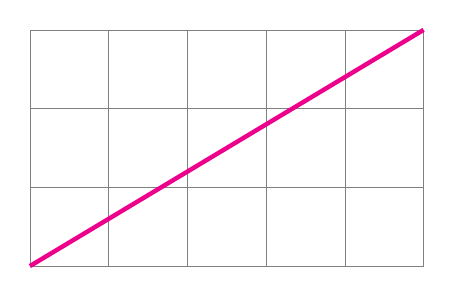
\begin{tikzpicture}
      \draw[step=1.0cm,gray,very thin] (0,0) grid (5,3);
      \draw[magenta,ultra thick] (0,0) -- (5,3);
    \end{tikzpicture}
  \end{minipage}
  \hfill
  \begin{minipage}{0.31\textwidth}
    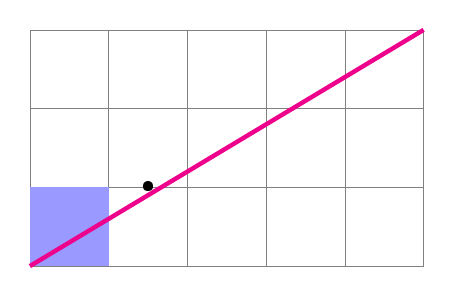
\begin{tikzpicture}
      \draw[step=1.0cm,gray,very thin] (0,0) grid (5,3);
      \fill[blue!40!white] (0,0) rectangle (1,1);
      \draw[magenta,ultra thick] (0,0) -- (5,3);
      \node at (1.5,1) {\textbullet};
    \end{tikzpicture}
  \end{minipage}
  \hfill
  \begin{minipage}{0.31\textwidth}
    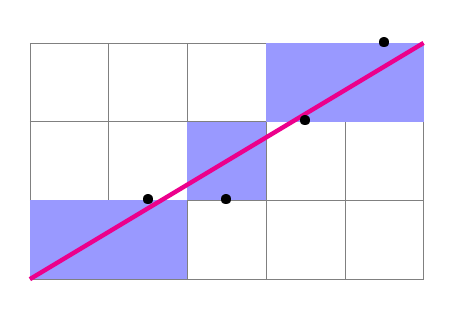
\begin{tikzpicture}
      \draw[step=1.0cm,gray,very thin] (0,0) grid (5,3);
      \fill[blue!40!white] (0,0) rectangle (1,1);
      \fill[blue!40!white] (1,0) rectangle (2,1);
      \fill[blue!40!white] (2,1) rectangle (3,2);
      \fill[blue!40!white] (3,2) rectangle (4,3);
      \fill[blue!40!white] (4,2) rectangle (5,3);
      \draw[magenta,ultra thick] (0,0) -- (5,3);
      \node at (1.5,1) {\textbullet};
      \node at (2.5,1) {\textbullet};
      \node at (3.5,2) {\textbullet};
      \node at (4.5,3) {\textbullet};
    \end{tikzpicture}
  \end{minipage}
  \caption{\label{fig:oct1} Plotting a line in octant I.}
\end{figure}

We start with the leftmost column (i.e., the smallest $x$-value) and work our way up.
Earlier on, we said that $x_0$ and $y_0$ are integers, so we can begin by plotting point $(x_0, y_0)$ (see the middle graph of Figure~\ref{fig:oct1}).

Since we are strictly moving from left to right and down to up, we must move onto the next column.
From here, we have two (logical) choices.
Do we fill in $(x_0 + 1, y_0)$ or $(x_0 + 1, y_0 + 1)$?
It turns out that we can actually figure this out with minimal work.
All lines are functions that can be expressed in the form $y_i = f(x_i)$.
So for a given $x_i$-value, we can calculate the corresponding $y_i$-value.
Then, we compare that calculated $y_i$ value to the \enquote{midway} value $y_j = f\left(x_i + \frac{1}{2}\right)$ to see which pixel contains \enquote{more} of the line.
We can express this like so:

\begin{quote}
  If $\left(x + 1, y + \frac{1}{2}\right)$ is above the line, draw the lower pixel.
  If it is below the line, draw the upper pixel.
  If it is exactly equivalent to the midpoint, pick either pixel.
\end{quote}

We avoid plotting two pixels for a single column so that the line does not turn thicker at various locations.

\subsection{Testing $\left(x + 1, y + \frac{1}{2}\right)$}
We can manipulate the point-slope equation $y = mx + b$ like so:
\begin{align*}
  0       &= mx - y + b \\
          &= \frac{\Delta y}{\Delta x} x - y + b \\
          &= (\Delta y) x - (\Delta x) y + (\Delta x) b \\
  f(x, y) &= Ax + By + C
\end{align*}
In this case, $A = \Delta y$, $B = -\Delta x$, and $C = \Delta x$.
This gives us the first draft of our algorithm, written in psuedo-code:
\begin{lstlisting}[mathescape]
  $x = x_0$; $y = y_0$
  $d = f\left(x + 1, y + \frac{1}{2}\right)$
  while $x \leq x_1$
    plot($x$, $y$)
    $x$++
    if $d > 0$ then $y$++
    $d = f\left(x + 1, y + \frac{1}{2}\right)$
\end{lstlisting}
We realize that if $x$ increases by 1, add $A$ to $d$, and if $y$ increases by 1, add $B$ to $d$.
We can revise the algorithm to get our second draft (diff-mode below):
\begin{lstlisting}[mathescape]
   $x = x_0$; $y = y_0$
   $d = f\left(x + 1, y + \frac{1}{2}\right)$
   while $x \leq x_1$
     plot($x$, $y$)
-    $x$++
+    $x$++; $d$ += $A$
-    if $d > 0$ then $y$++
+    if $d > 0$ then $y$++; $d$ += $B$
-    $d = f\left(x + 1, y + \frac{1}{2}\right)$
\end{lstlisting}
We can further simplify the value of $d$:
\begin{align*}
  d_0   &= f\left(x_0 + 1, y_0 + \frac{1}{2}\right) \\
        &= A(x_0 + 1) + B\left(y_0 + \frac{1}{2}\right) + C \\
        &= f(x_0, y_0) + A + \frac{1}{2} B \\
        &= A + \frac{1}{2} B \\
  2 d_0 &= 2A + B
\end{align*}
This gives us the third draft of the algorithm, which is more or less as optimized as it can be while avoiding division, which might return a floating-point number (diff-mode below):
\begin{lstlisting}[mathescape]
   $x = x_0$; $y = y_0$
-  $d = f\left(x + 1, y + \frac{1}{2}\right)$
+  $d = 2A + B$
   while $x \leq x_1$
     plot($x$, $y$)
-    $x$++; $d$ += $A$
+    $x$++; $d$ += $2A$
-    if $d > 0$ then $y$++; $d$ += $B$
+    if $d > 0$ then $y$++; $d$ += $2B$
\end{lstlisting}

\section{Octant II}
In octant II, we essentially just swap $x$- and $y$-values.
The midpoint becomes $\left(x + \frac{1}{2}, y + 1\right)$, and so $d_0 = f\left(x_0 + \frac{1}{2}, y + 1\right)$.
After simplification, we get $d = \frac{1}{2} A + B$, or $2d = A + 2B$.
The conditional $d > 0$ is flipped, and becomes $d < 0$.

\section{Octant VII}
Note that we have skipped many octants because one only has to flip octants I and II across the $y$-axis to obtain the formulas for octants III and IV, and across the origin for octants V and VI\@.
In octant VII, the midpoint is $\left(x + 1, y - \frac{1}{2}\right)$, and so $d_0 = f\left(x_0 + 1, y_0 - \frac{1}{2}\right)$.
After simplification, $2d = 2A - B$.

\end{document}
